
%---------------------------------------------------------------------------

\begin{frame}
\frametitle{Plan prezentacji}

\begin{enumerate}
\item Algorytm Scale Space
\item Przetwarzanie obrazów w~przestrzeni skali
\item Standard OpenCL
\item Dotychczasowe osiągnięcia
\end{enumerate}

\end{frame}

%---------------------------------------------------------------------------

\begin{frame}
\frametitle{Geneza algorytmu Scale Space}

Jednym z istotniejszych problemów podczas automatycznego przetwarzania i analizy obrazów jest wybór skali.

Obrazy mogą być rejestrowane w~różnych skalach.

\end{frame}

%---------------------------------------------------------------------------
\begin{frame}
\frametitle{Algorytm Scale Space}
\begin{block}{Scale Space}
Algorytm służący do przedstawiania sygnałów w reprezentacji skali.
\end{block}
Można go zastosować do dowolnych sygnałów. Praca skupia się na wykorzystaniu algorytmu do przetwarzania obrazów.

\end{frame}

%---------------------------------------------------------------------------
\begin{frame}
\frametitle{Podstawy matematyczne}
Do wyznaczenia przestrzeni skali stosuje się filtry Gaussa. Poniżej przedstawiono filtr w przestrzeni dwuwymiarowej.

\begin{center}
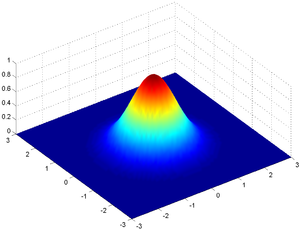
\includegraphics[width=3cm]{gaussian2d.png}

$ g(x,y,\sigma)= \frac{1}{2 \cdot \pi \cdot \sigma ^ {2} }\cdot e^{(-\frac{x^{2} + y^{2}}{2 \cdot \sigma ^{2}})} $
\end{center}
\end{frame}
%---------------------------------------------------------------------------
\begin{frame}
\frametitle{Algorytm Scale Space dla obrazów}


\begin{figure}[h]
\begin{center}
\begin{subfigure}[b]{2cm}
                 \centering
                 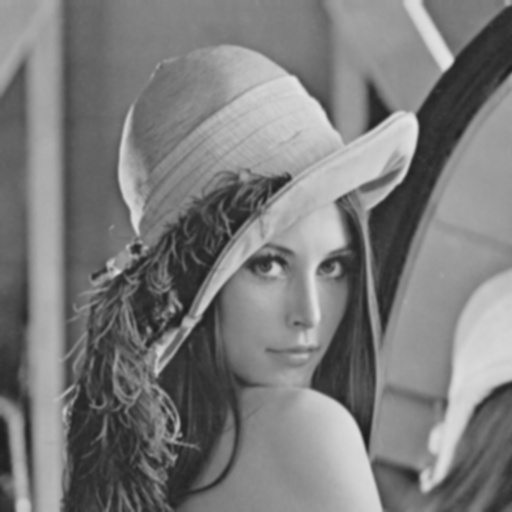
\includegraphics[width=2cm]{Lena_scales1.jpg}
         \end{subfigure}%
		 ~
\begin{subfigure}[b]{2cm}
                 \centering
                 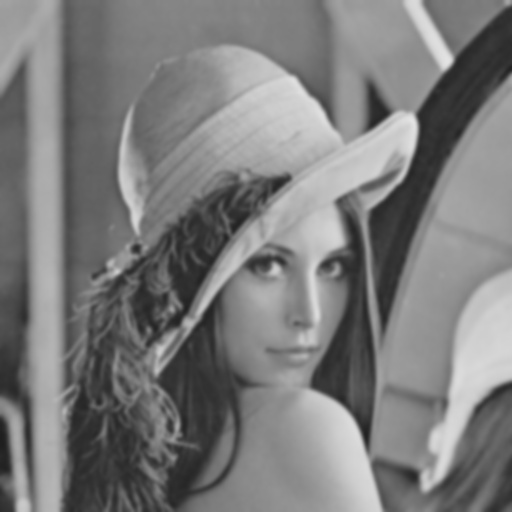
\includegraphics[width=2cm]{Lena_scales2.jpg}
         \end{subfigure}%
		 ~
\begin{subfigure}[b]{2cm}
                 \centering
                 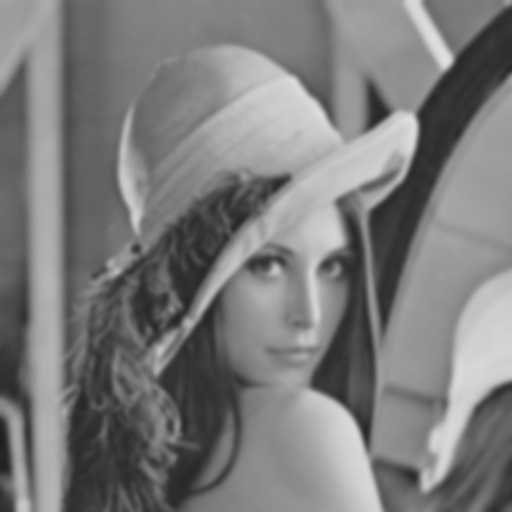
\includegraphics[width=2cm]{Lena_scales3.jpg}
         \end{subfigure}%
		 
		 
\begin{subfigure}[b]{2cm}
                 \centering
                 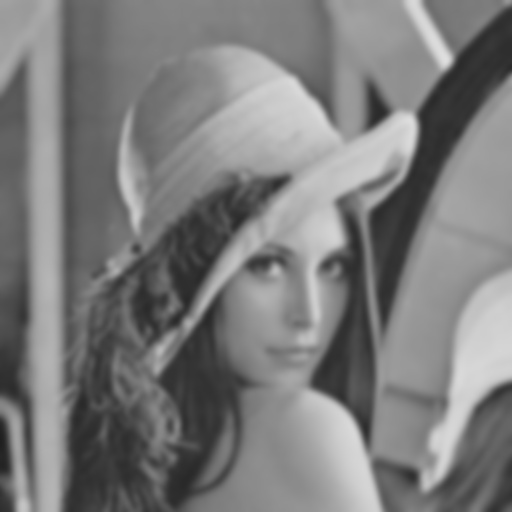
\includegraphics[width=2cm]{Lena_scales4.jpg}
         \end{subfigure}%
		 ~
		 \begin{subfigure}[b]{2cm}
                 \centering
                 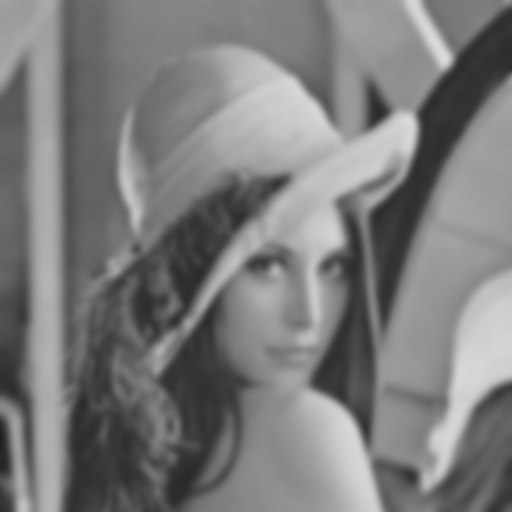
\includegraphics[width=2cm]{Lena_scales5.jpg}
         \end{subfigure}%
		 ~
\begin{subfigure}[b]{2cm}
                 \centering
                 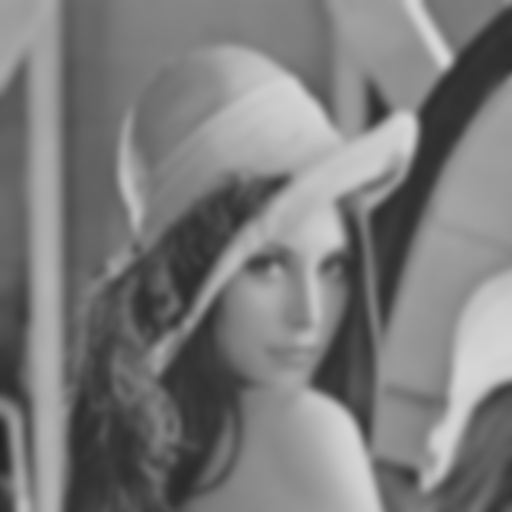
\includegraphics[width=2cm]{Lena_scales6.jpg}
         \end{subfigure}%
\caption{Obraz w przestrzeni skali}
\label{lena_scales}
\end{center}
\end{figure}
\end{frame}


%---------------------------------------------------------------------------
\begin{frame}
\frametitle{Przetwarzanie obrazów w przestrzeni skali}

Po wyznaczeniu reprezentacji skali dla obrazu można przeprowadzić dalsze operacje, w zależności od ustalonego celu. Przykładowe cele:
\begin{itemize}
\item rozpoznawanie plam,
\item rozpoznawanie krawędzi,
\item rozpoznawanie innych struktur.
\end{itemize}
Dzięki temu, że obraz jest przetwarzany w~różnych skalach, można rozpoznawać dane struktury dla różnych stopni szczegółowości.
\end{frame}

%---------------------------------------------------------------------------
\begin{frame}
\frametitle{OpenCL}
\begin{block}{OpenCL}
Otwarty, wieloplatformowy standard pozwalający na wykorzystanie procesorów kart graficznych oraz innych urządzeń w celu wykonywania obliczeń ogólnego przeznaczenia.
\end{block}

Dzięki temu można zrównoleglać obliczenia, co przyśpiesza ich wykonywanie.

\end{frame}


%---------------------------------------------------------------------------
\begin{frame}
\frametitle{Wykorzystanie OpenCL}

Do implementacji algorytmu z~wykorzystaniem OpenCL konieczne jest:
\begin{itemize}
\item Napisanie kodu kerneli - fragmentów kodu wykonywanych na karcie graficznej.
\item Napisanie kodu wykonywanego na procesorze, który będzie kontrolował część wykonywaną na karcie graficznej. W tym zawiera się przekazanie parametrów do kerneli oraz pobranie wyników.
\end{itemize}

\end{frame}


%---------------------------------------------------------------------------
\begin{frame}
\frametitle{Dotychczas zrealizowane zadania}

Do tej pory udało się zrealizować:
\begin{itemize}
\item szkielet (bibliotekę), ułatwiający implementację kerneli,
\item kernel realizujący konwolucję - używany z filtrami Gaussa,
\item kernele realizujące rozpoznawanie plam (blobs)*.
\end{itemize}

\end{frame}


%---------------------------------------------------------------------------
\begin{frame}
\frametitle{Rozpoznawanie plam}

Po wyznaczeniu reprezentacji skali obrazu wykorzystuje się operator Laplace'a.
\begin{center}
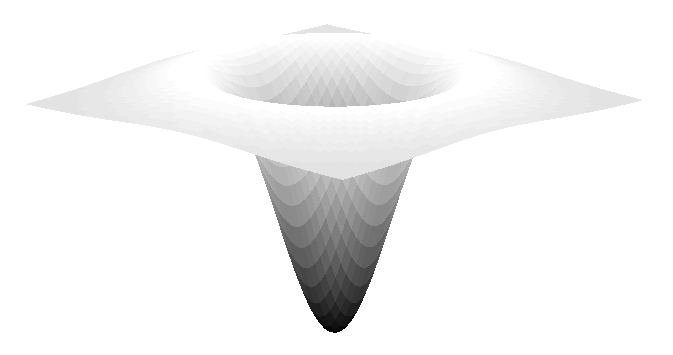
\includegraphics[width=3cm]{laplacian.png}
\end{center}
Jest on stosowany do całej reprezentacji skali. Następnie wyznaczane są maksima (lub minima) w otrzymanej trójwymiarowej strukturze.

\end{frame}
%---------------------------------------------------------------------------
\begin{frame}
\frametitle{Rozpoznawanie plam - przykład}

\begin{figure}[h]
\begin{center}
\begin{subfigure}[b]{2cm}
                 \centering
                 
\includegraphics[width=2cm]{original.jpg}
         \end{subfigure}%
		 ~
\begin{subfigure}[b]{2cm}
\centering
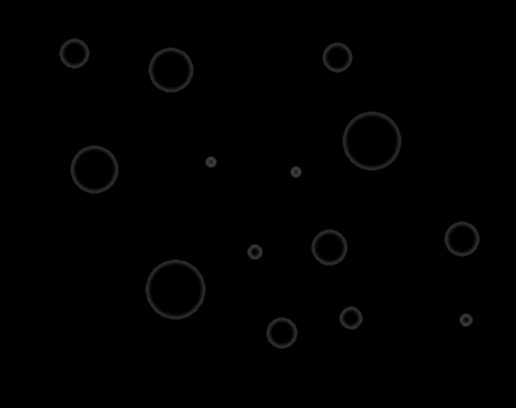
\includegraphics[width=2cm]{circles1.jpg}
\end{subfigure}~
\begin{subfigure}[b]{2cm}
\centering
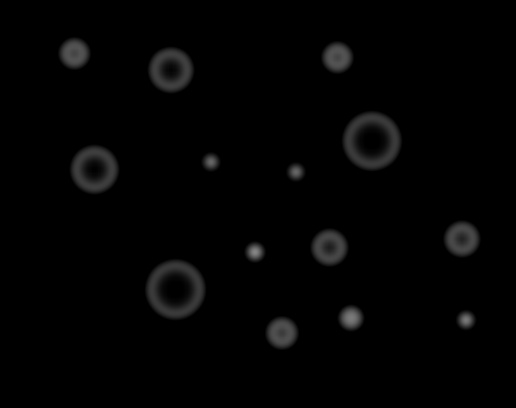
\includegraphics[width=2cm]{circles2.jpg}
\end{subfigure}~
\begin{subfigure}[b]{2cm}
\centering
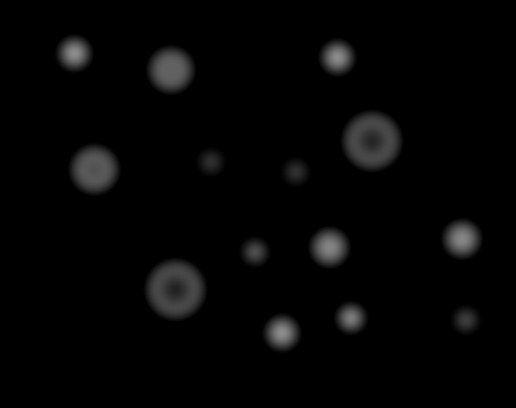
\includegraphics[width=2cm]{circles3.jpg}
\end{subfigure}


\begin{subfigure}[b]{2cm}
\centering
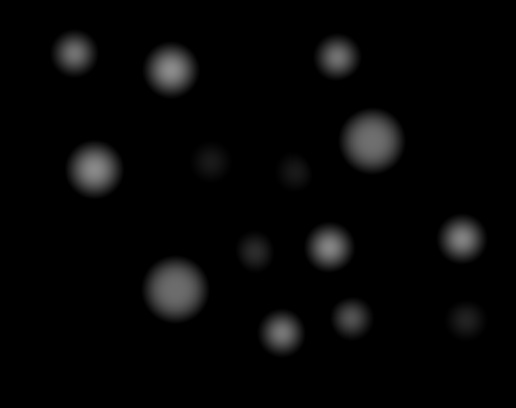
\includegraphics[width=2cm]{circles4.jpg}
\end{subfigure}~
\begin{subfigure}[b]{2cm}
\centering
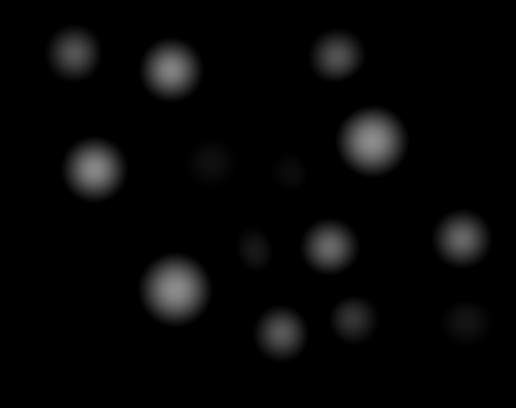
\includegraphics[width=2cm]{circles5.jpg}
\end{subfigure}~
\begin{subfigure}[b]{2cm}
\centering

\includegraphics[width=2cm]{circles6.jpg}
\end{subfigure}~
\begin{subfigure}[b]{2cm}
\centering
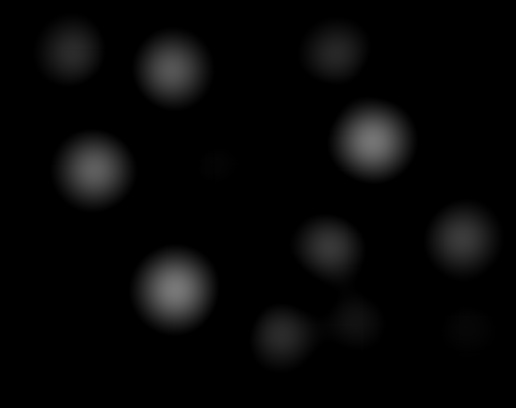
\includegraphics[width=2cm]{circles7.jpg}
\end{subfigure}
\caption{Wynik przetworzenia obrazów w reprezentacji skali operatorem Laplace'a}
\label{circles}
\end{center}
\end{figure}

\end{frame}

%---------------------------------------------------------------------------
\begin{frame}
\frametitle{Znalezione plamy}
\begin{figure}
\begin{center}
\begin{subfigure}[b]{5cm}
\centering

\includegraphics[width=5cm]{outp.png}
\end{subfigure}~
\begin{subfigure}[b]{5cm}
\centering

\includegraphics[width=5cm]{result.png}
\end{subfigure}
\end{center}
\caption{Znalezione plamy są zaznaczone szarym okręgiem.}
\end{figure}
\end{frame}

%---------------------------------------------------------------------------
\begin{frame}
\frametitle{}
\begin{center}
Dziękuję za uwagę.
\end{center}
\end{frame}